\documentclass[11pt]{article}

\usepackage[margin=1in]{geometry}
\usepackage{booktabs}
\usepackage{graphicx}
\usepackage{float}
\usepackage{caption}
\usepackage{subcaption}
\usepackage{array}
\usepackage{hyperref}

\hypersetup{
  colorlinks=true,
  linkcolor=black,
  citecolor=black,
  urlcolor=black
}

\title{Revised Dynamic Emotion Simulation Benchmark}
\author{}
\date{\today}

\begin{document}
\maketitle

\section{Overview}

This brief report summarizes the revised first-simulation benchmark comparing
DynEGA, GraphicalVAR, and GIMME on simulated dynamic emotion panels. The revised
benchmark uses the old first-simulation design logic but replaces the original
simulation scenarios with the newer dynamic latent-factor scenarios. DynEGA and
GraphicalVAR are evaluated on the main full grid. GIMME is reported separately as
a bounded feasibility comparator because full-grid GIMME estimation was not
computationally tractable under the same design.

\section{Simulation Benchmark Results}

The main full-grid comparison contains 1,920 benchmark rows per method for
DynEGA and GraphicalVAR. GIMME is limited to a 120-row bounded feasibility grid.
Table~\ref{tab:benchmark-overview} gives the standard benchmark metrics from
the completed comparison run.

\begin{table}[H]
\centering
\caption{Method-level benchmark overview. Exact recovery is the proportion of
conditions in which the recovered dimensionality matched the generating
structure. Runtime is mean wall-clock time per benchmark row.}
\label{tab:benchmark-overview}
\small
\begin{tabular}{lrrrrrrrrr}
\toprule
Method & Scope & Runs & Success & Timeout & Error & Exact & Cor. & NRMSE & Runtime \\
\midrule
DynEGA & Full grid & 1920 & 1.000 & 0 & 0 & 0.974 & 0.654 & 0.867 & 3.6 s \\
GraphicalVAR & Full grid & 1920 & 0.975 & 48 & 0 & 0.873 & 0.649 & 0.865 & 191.4 s \\
GIMME & Bounded & 120 & 0.175 & 96 & 3 & 0.158 & 0.614 & 0.944 & 364.3 s \\
\bottomrule
\end{tabular}
\end{table}

DynEGA is the most robust method in this benchmark. It completed all full-grid
conditions, recovered the correct number of dimensions in 97.4\% of rows, and
had the highest score assignment accuracy. GraphicalVAR produced similar score
correlations and slightly lower NRMSE, but this came at much higher runtime and
with 48 full-grid timeouts. GIMME recovered dimensionality reasonably often only
conditional on completion, but its all-row performance was dominated by timeouts
and errors.

\begin{figure}[H]
\centering
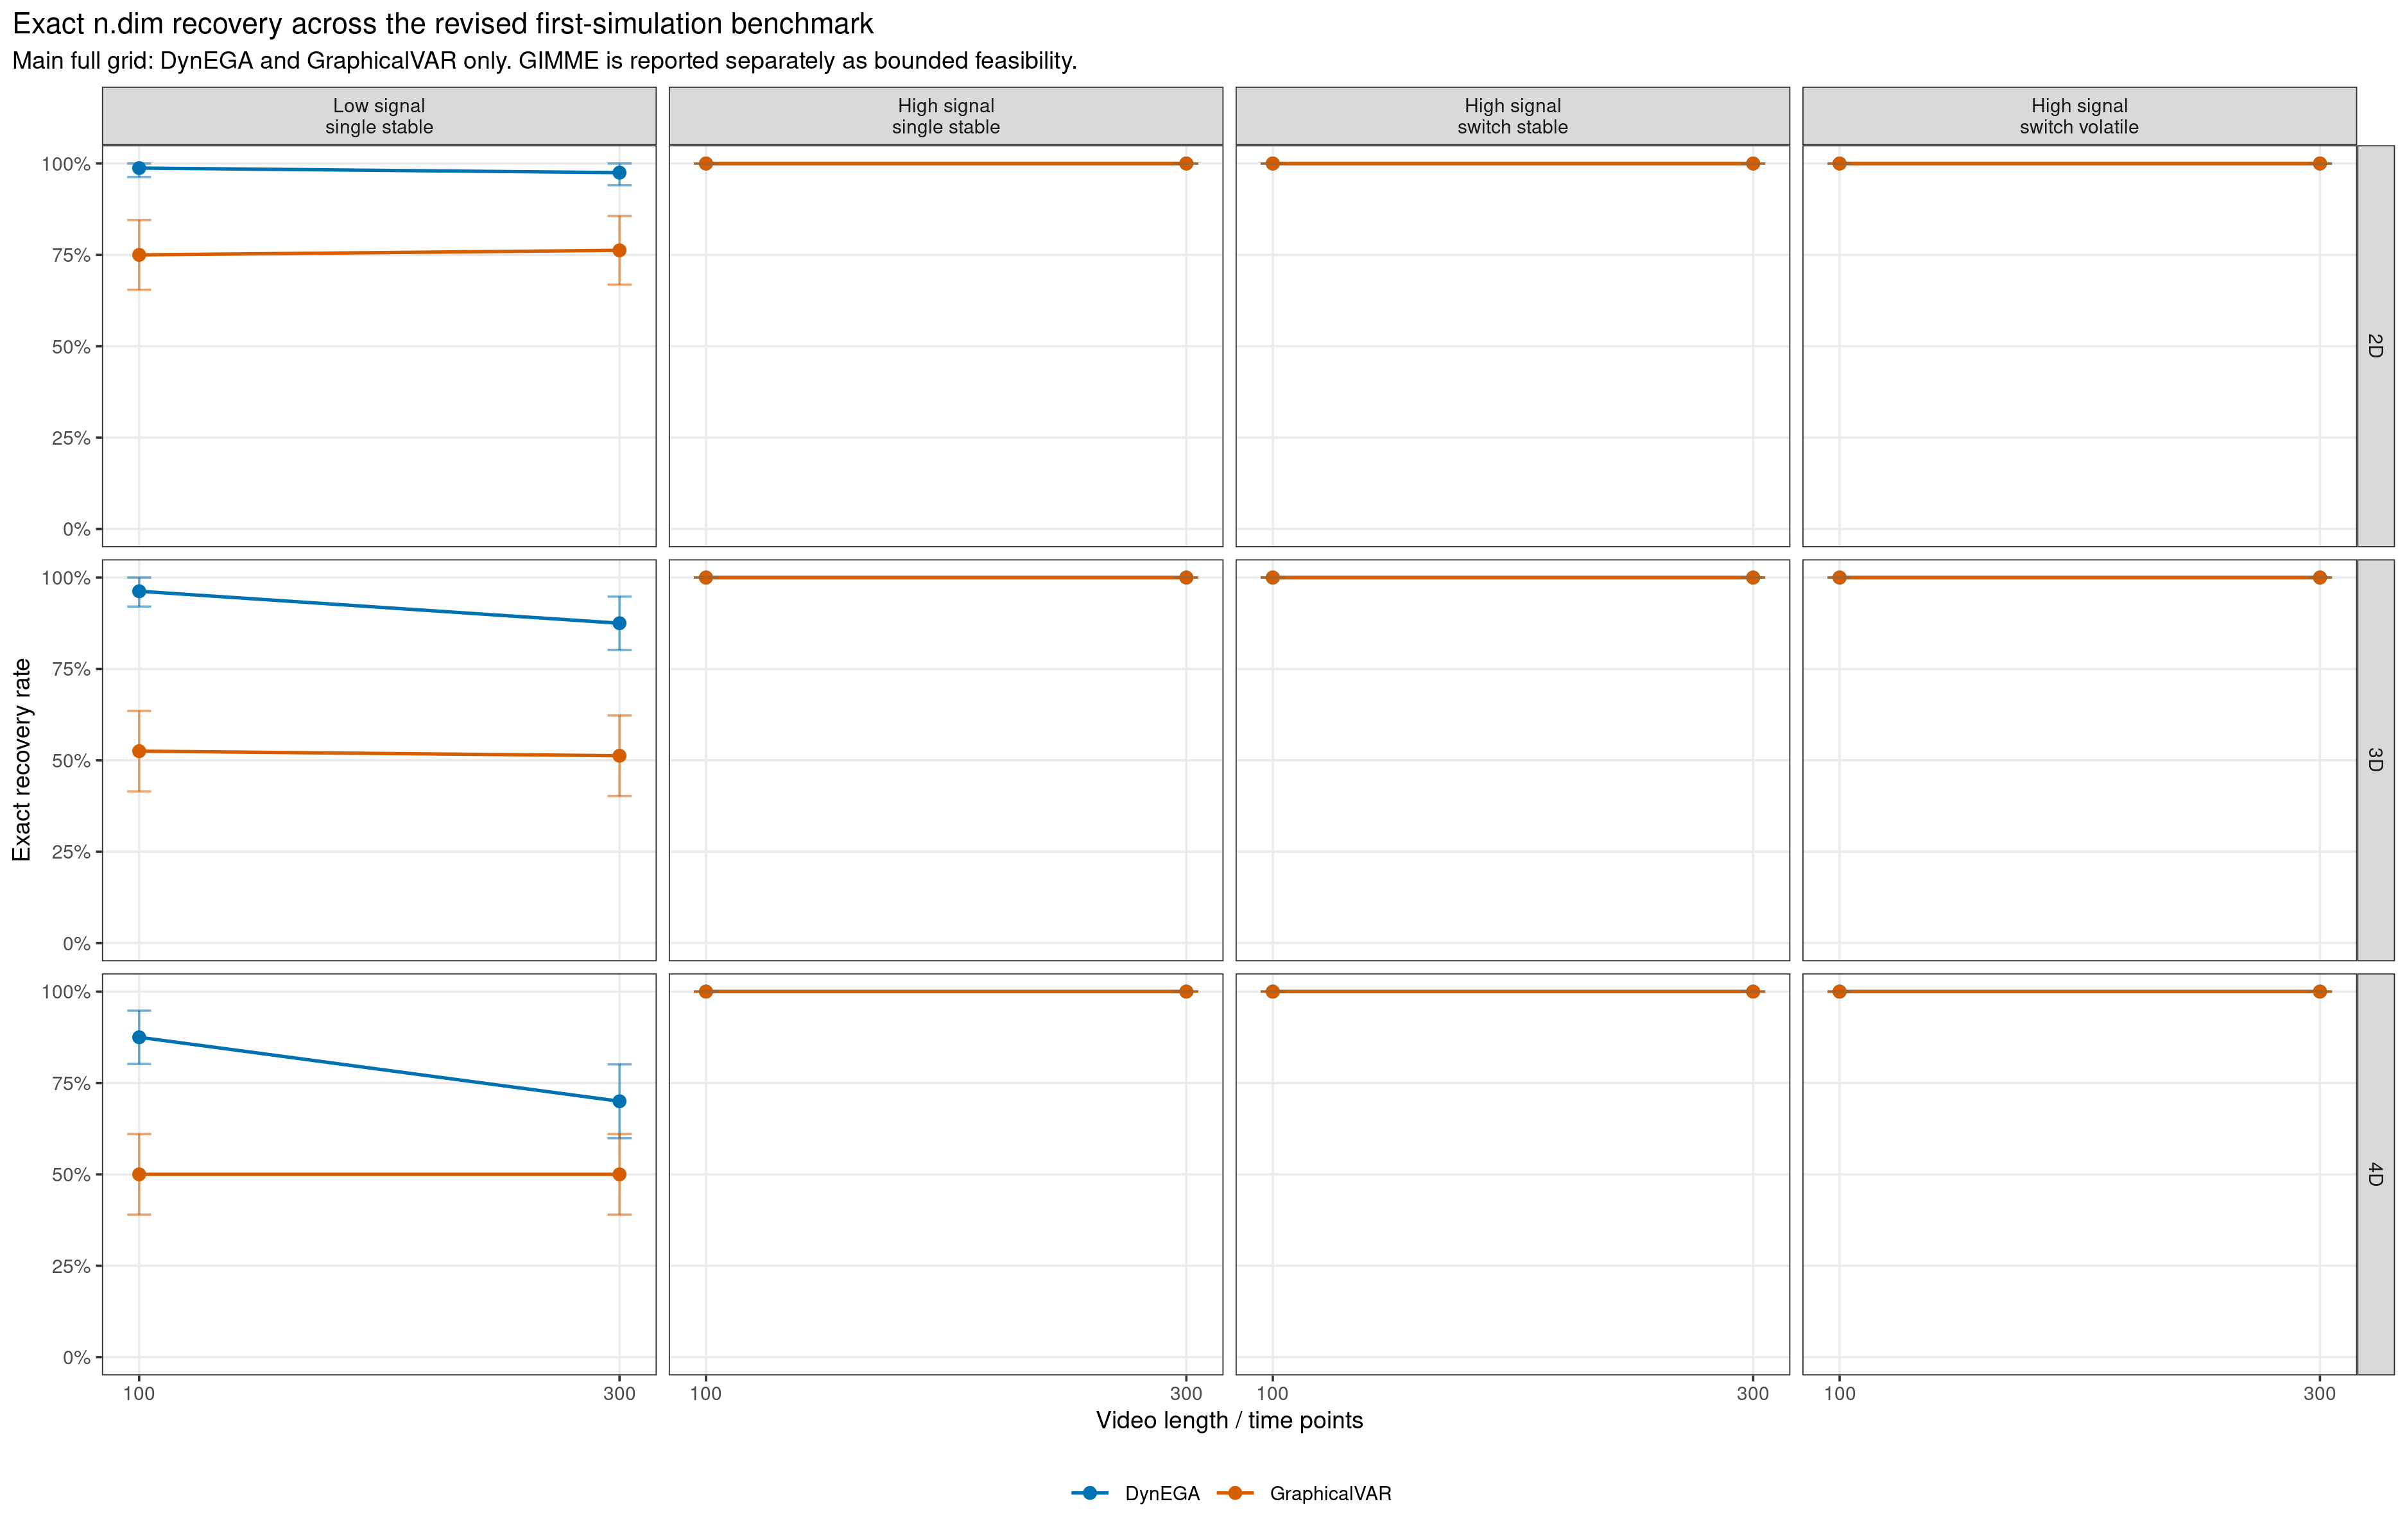
\includegraphics[width=0.92\linewidth]{comparison_revision_first_benchmark/01_hit_rate_by_timep.png}
\caption{Exact dimensional recovery by time-series length.}
\label{fig:hit-rate}
\end{figure}

\begin{figure}[H]
\centering
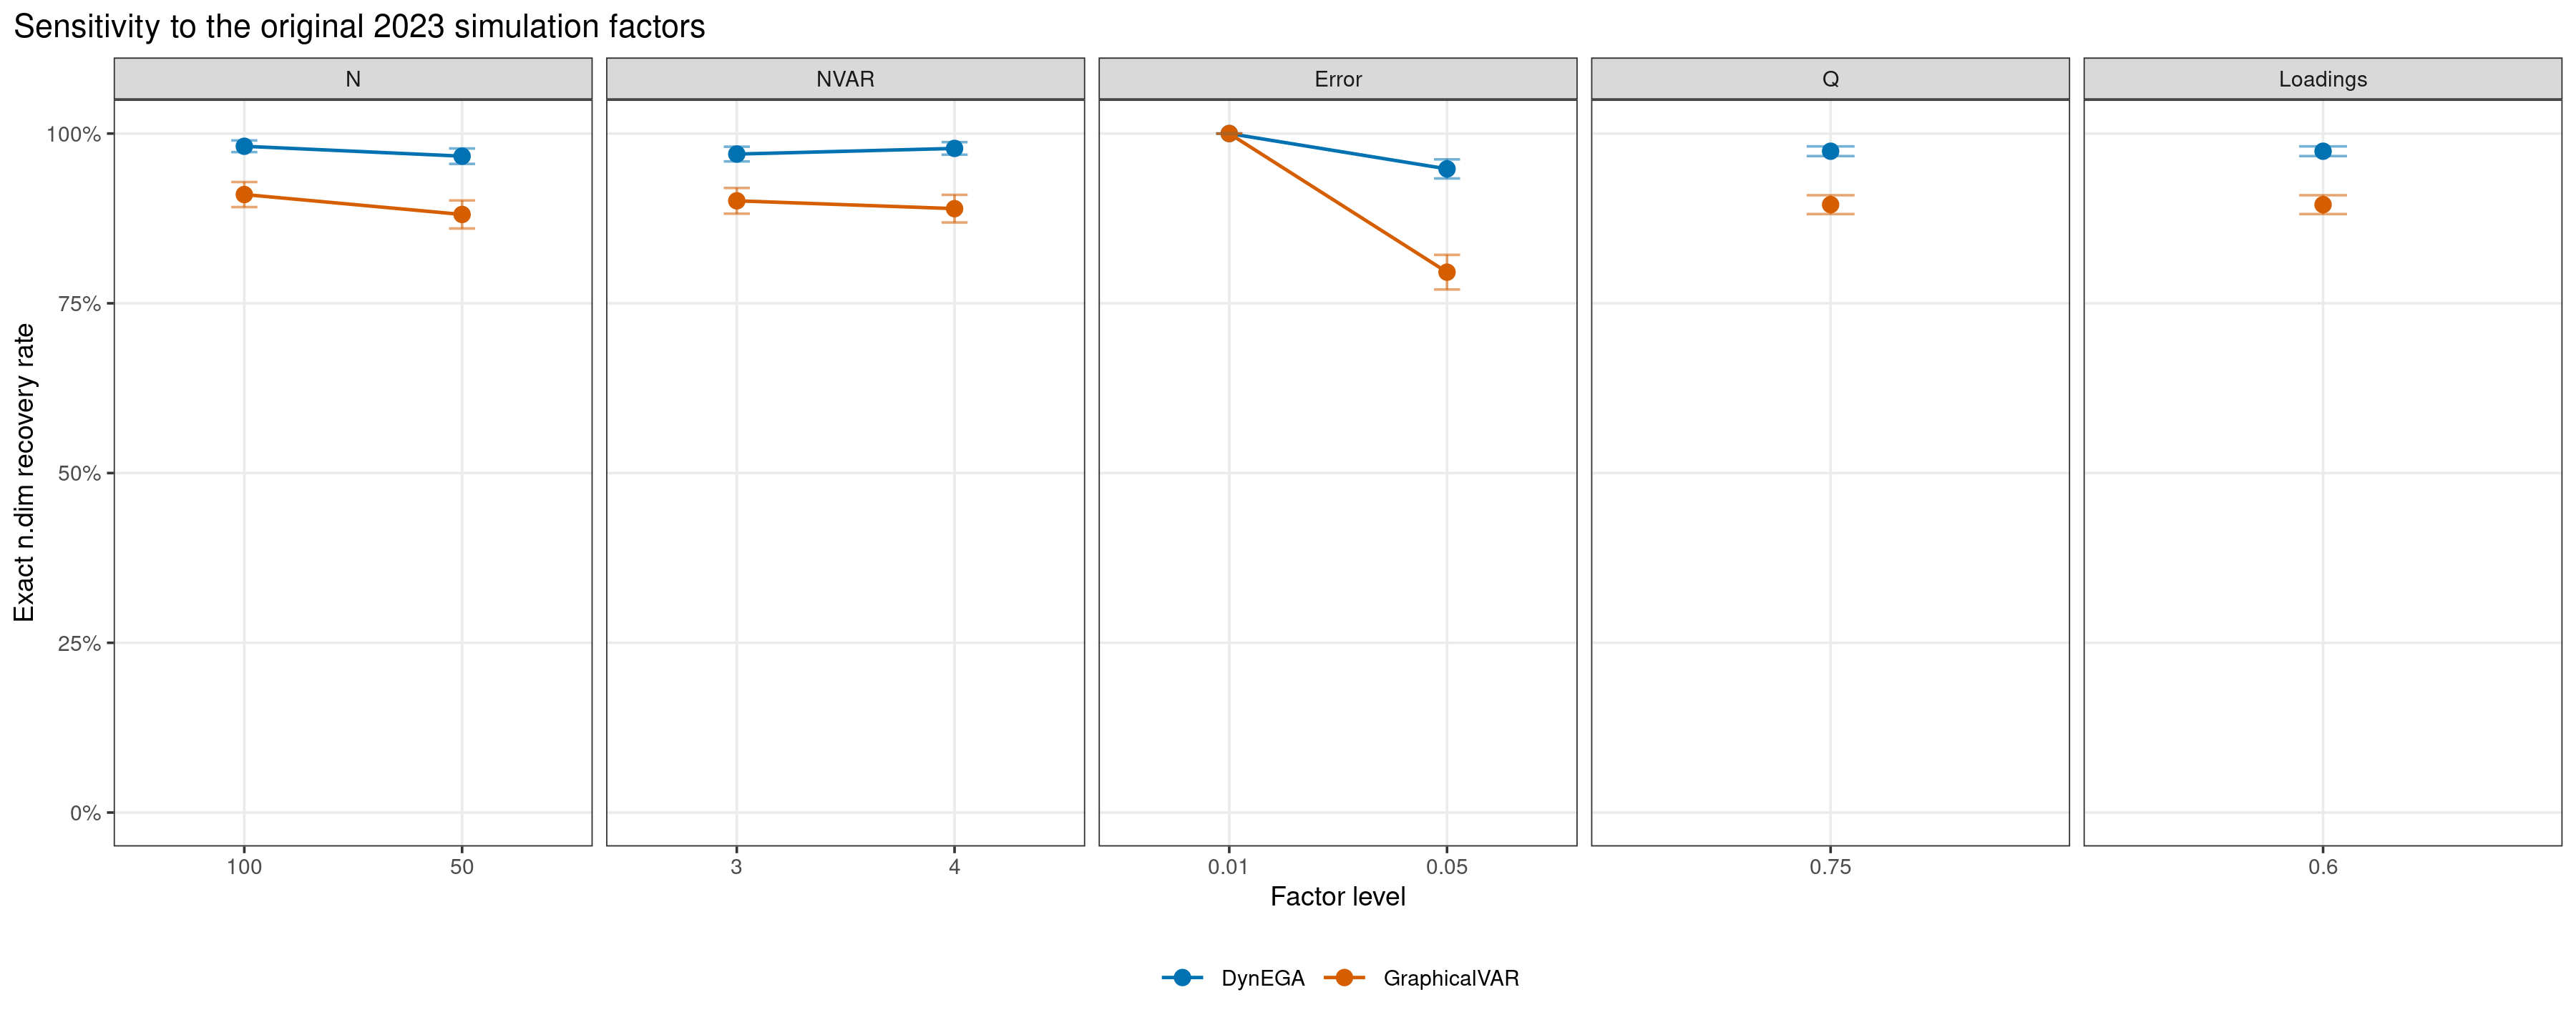
\includegraphics[width=0.92\linewidth]{comparison_revision_first_benchmark/02_old_factor_sensitivity.png}
\caption{Sensitivity of recovery to the first-simulation design factors.}
\label{fig:old-factor-sensitivity}
\end{figure}

\begin{figure}[H]
\centering
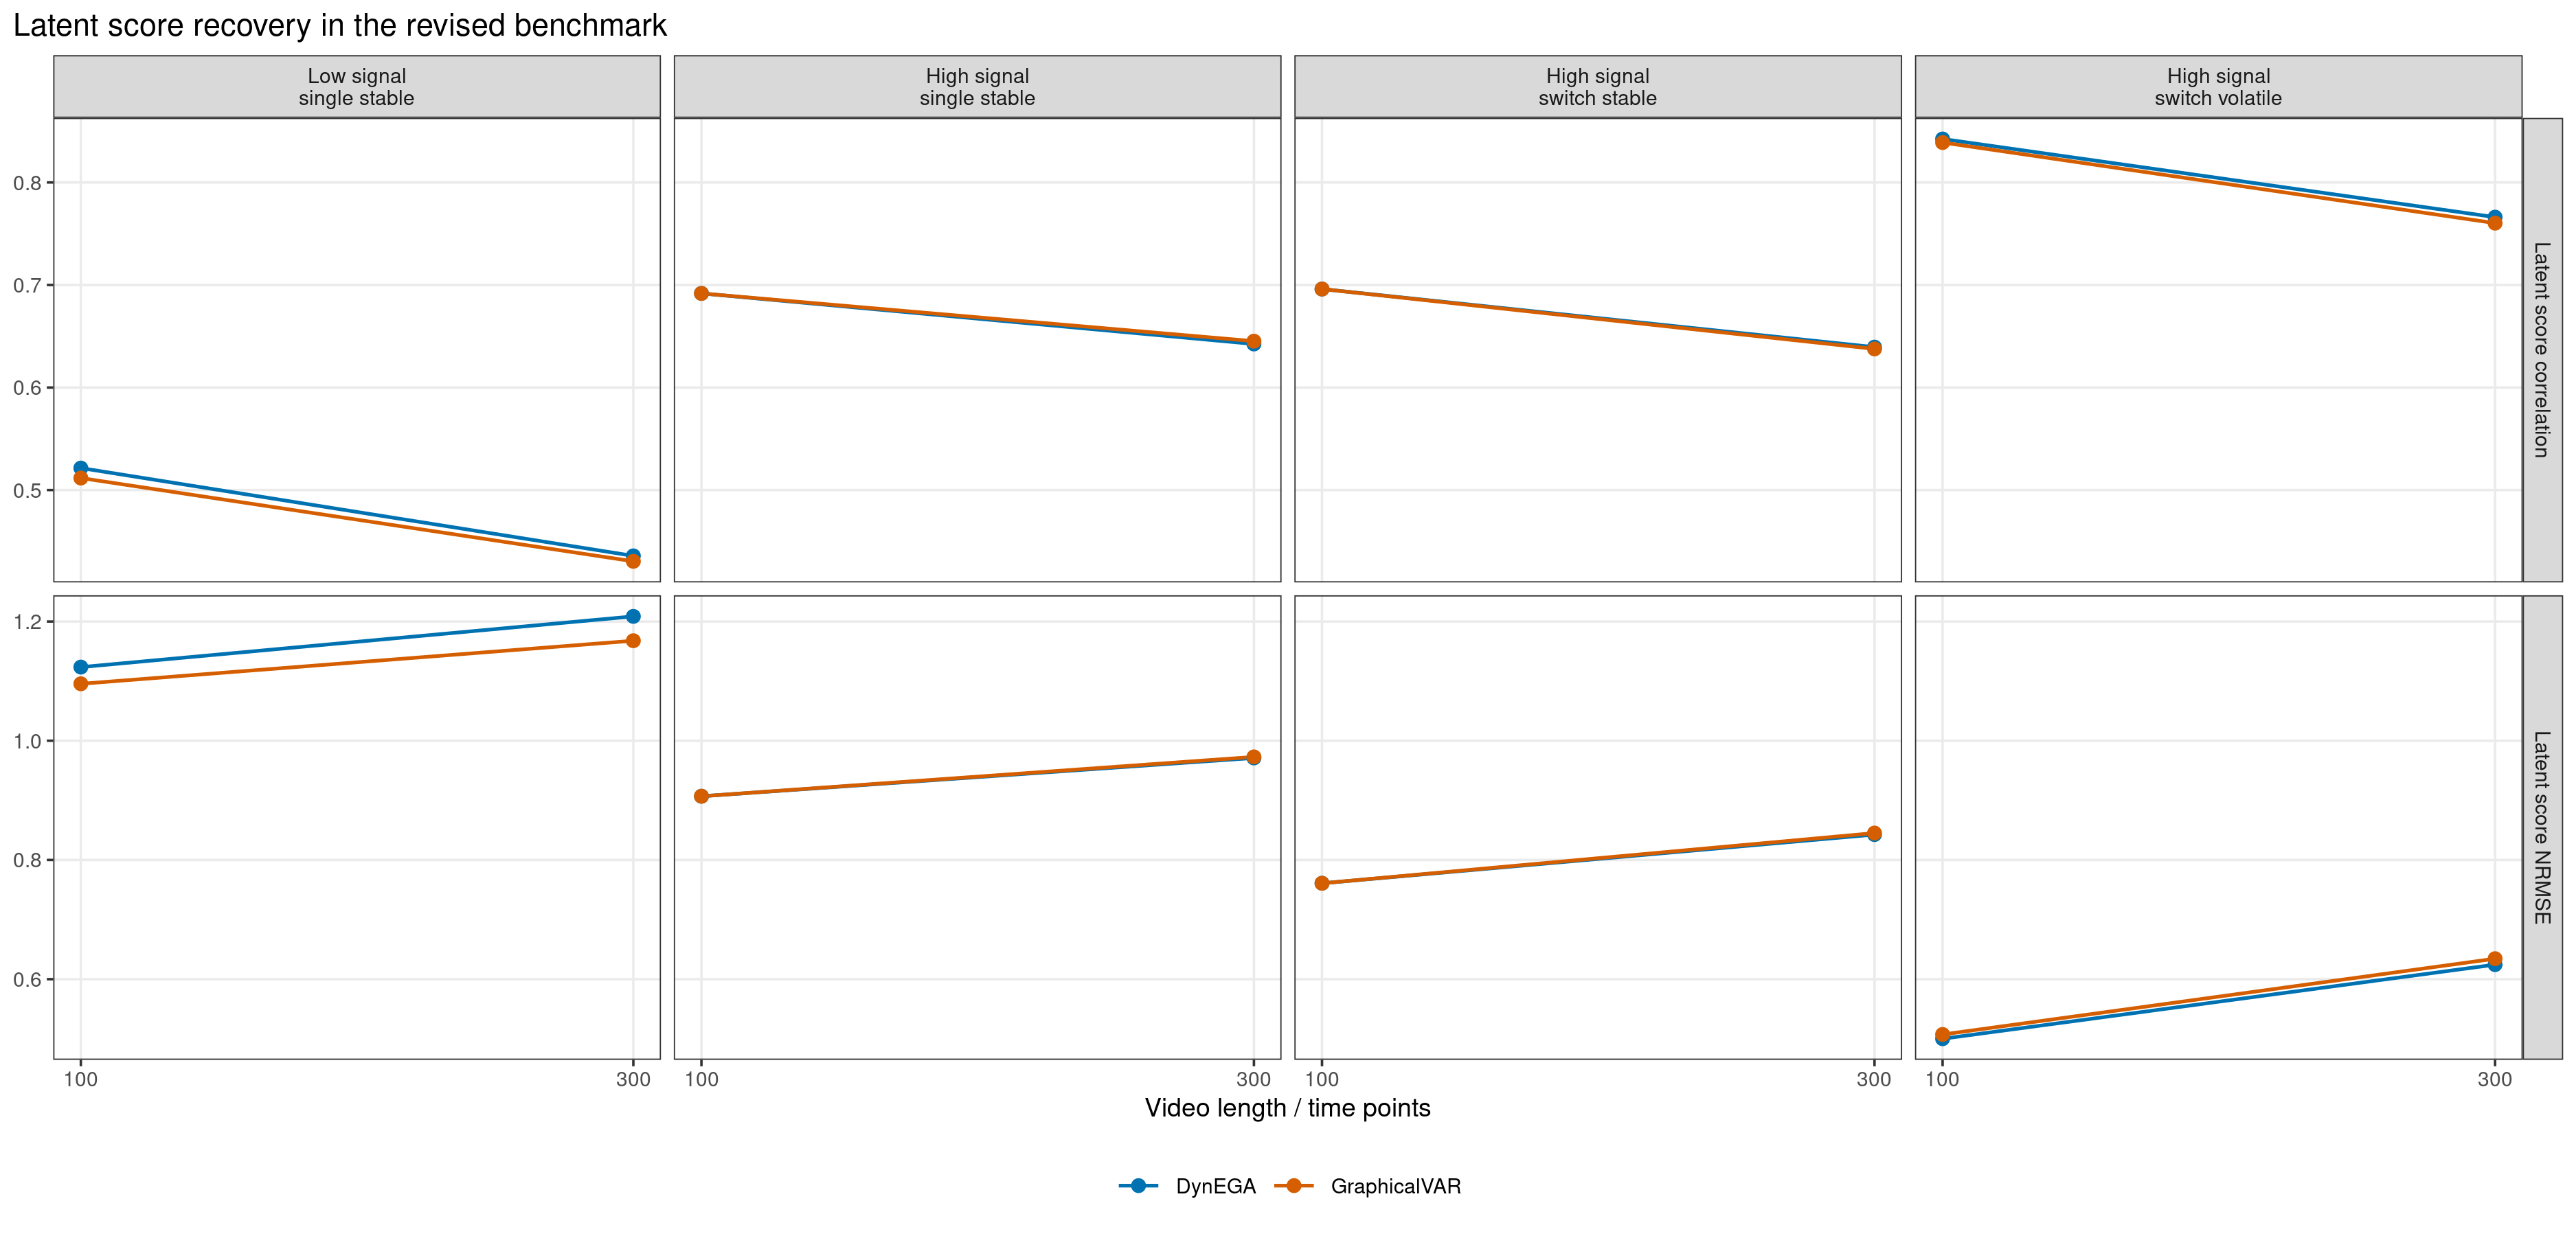
\includegraphics[width=0.92\linewidth]{comparison_revision_first_benchmark/03_score_recovery.png}
\caption{Recovery of latent score structure by method and scenario.}
\label{fig:score-recovery}
\end{figure}

\begin{figure}[H]
\centering
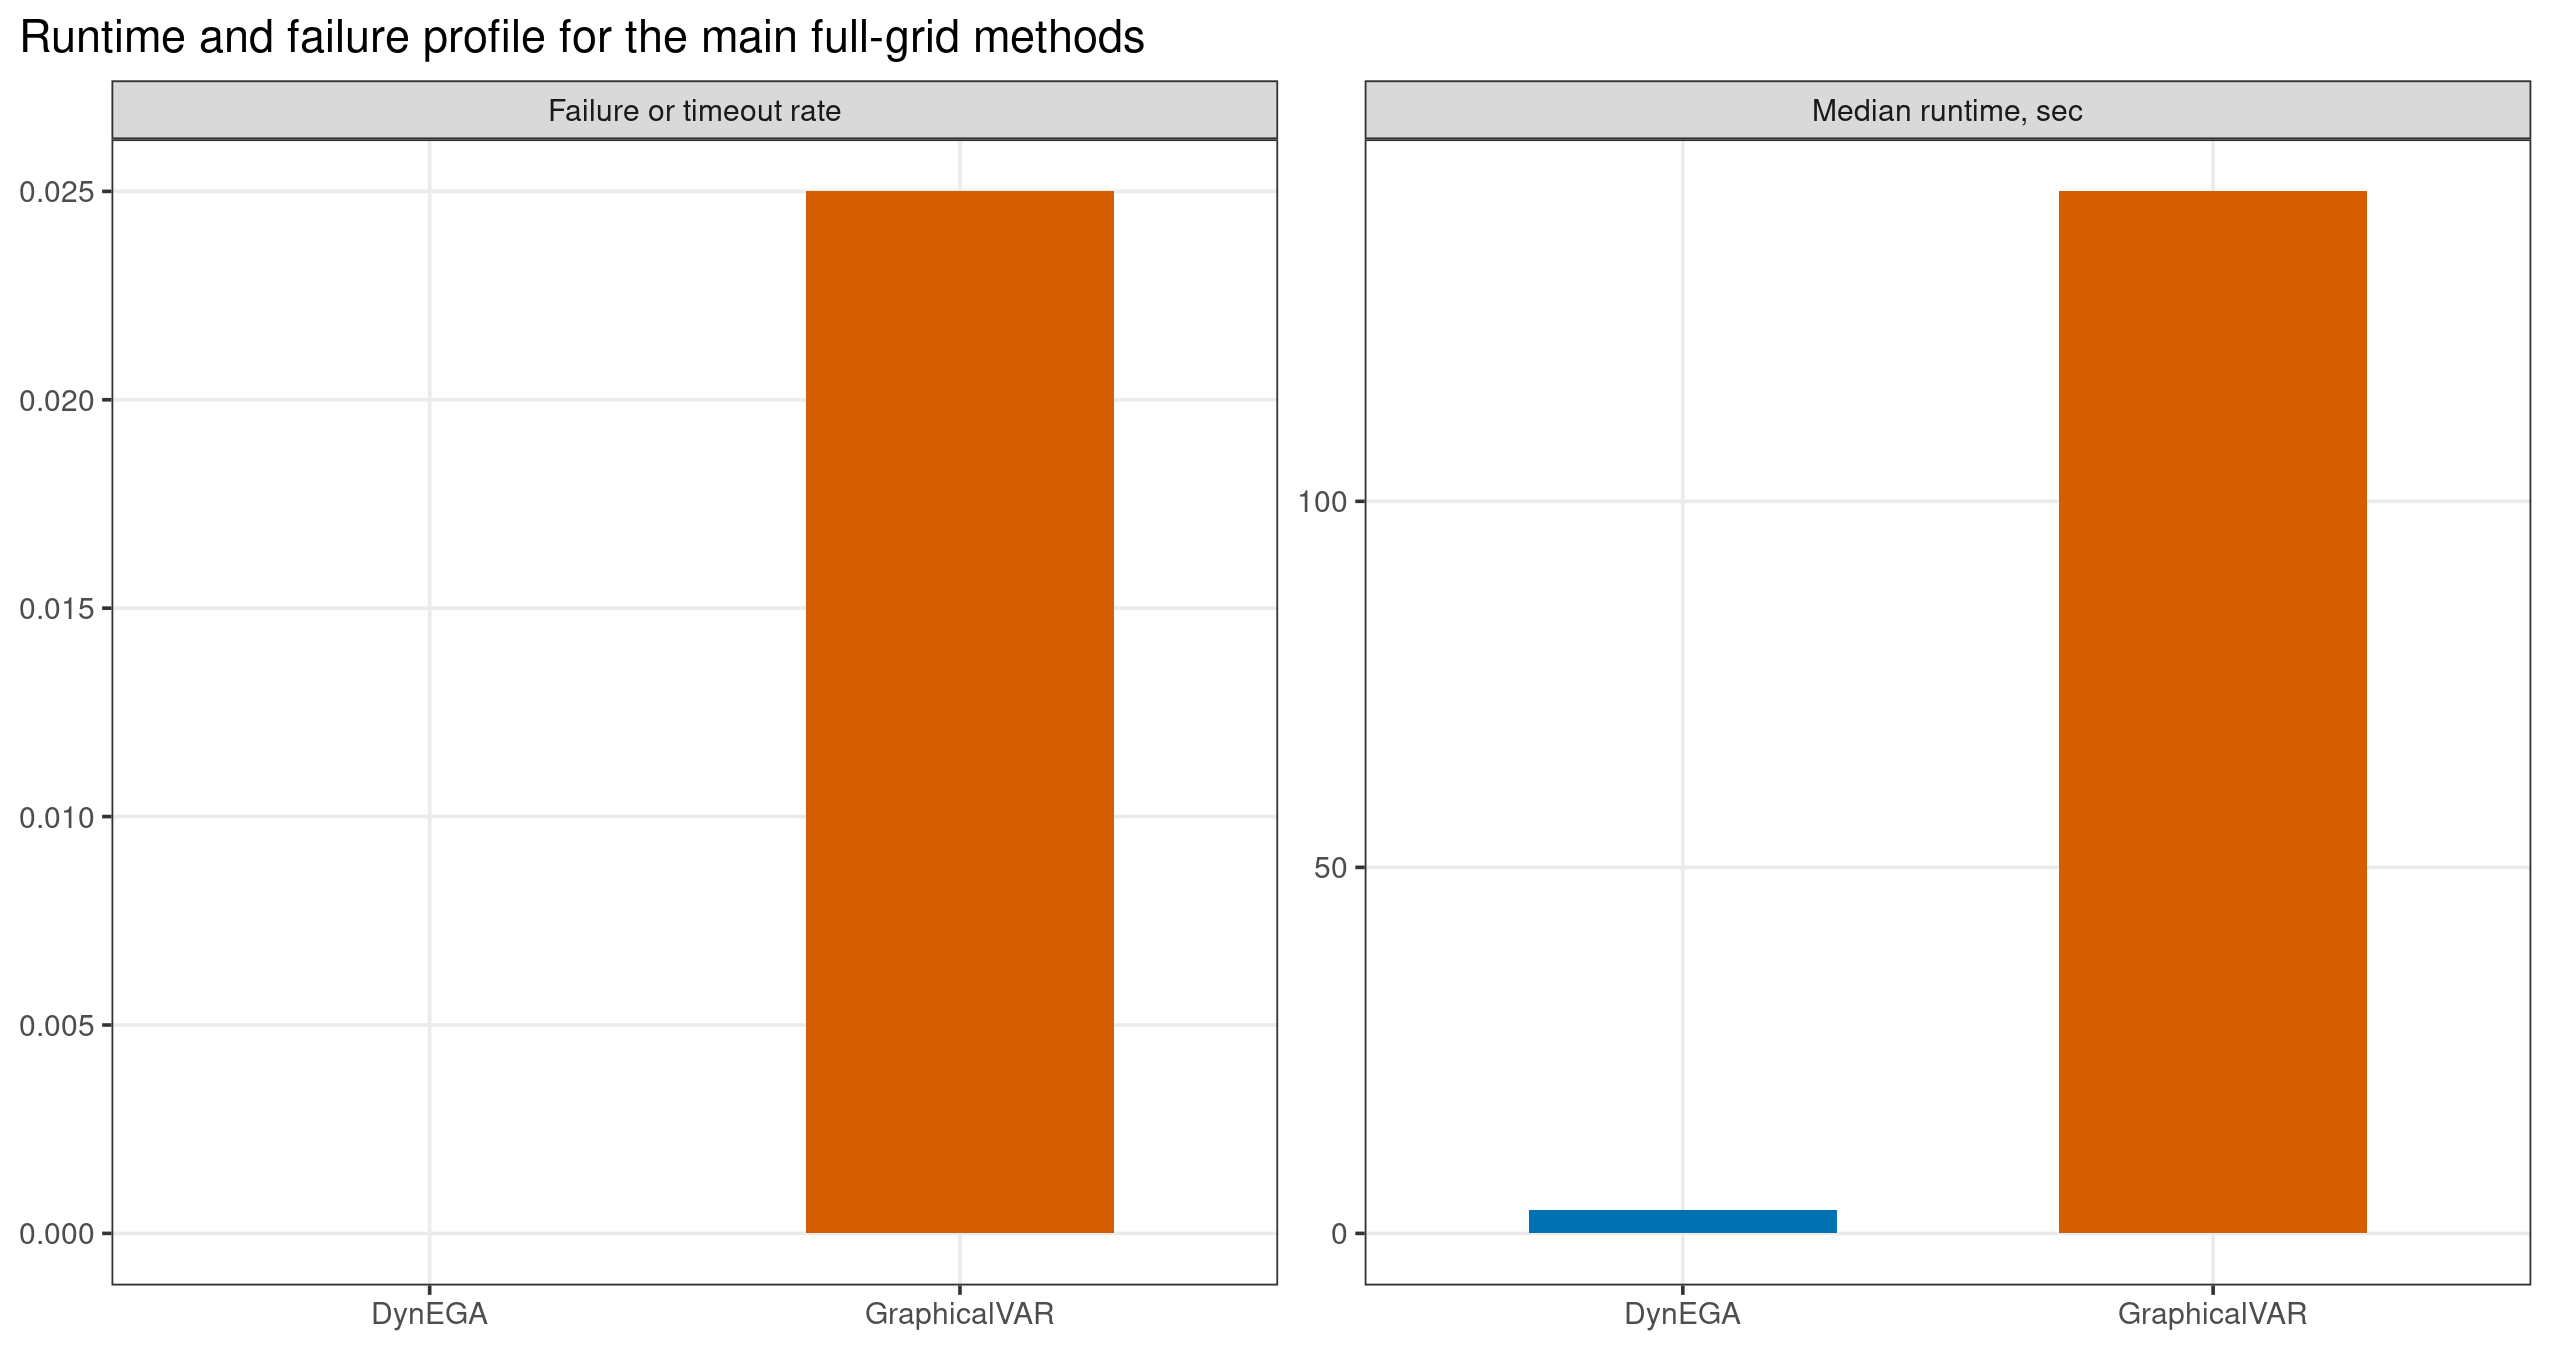
\includegraphics[width=0.92\linewidth]{comparison_revision_first_benchmark/04_runtime_and_failures.png}
\caption{Runtime and failure accounting.}
\label{fig:runtime-failures}
\end{figure}

\begin{figure}[H]
\centering
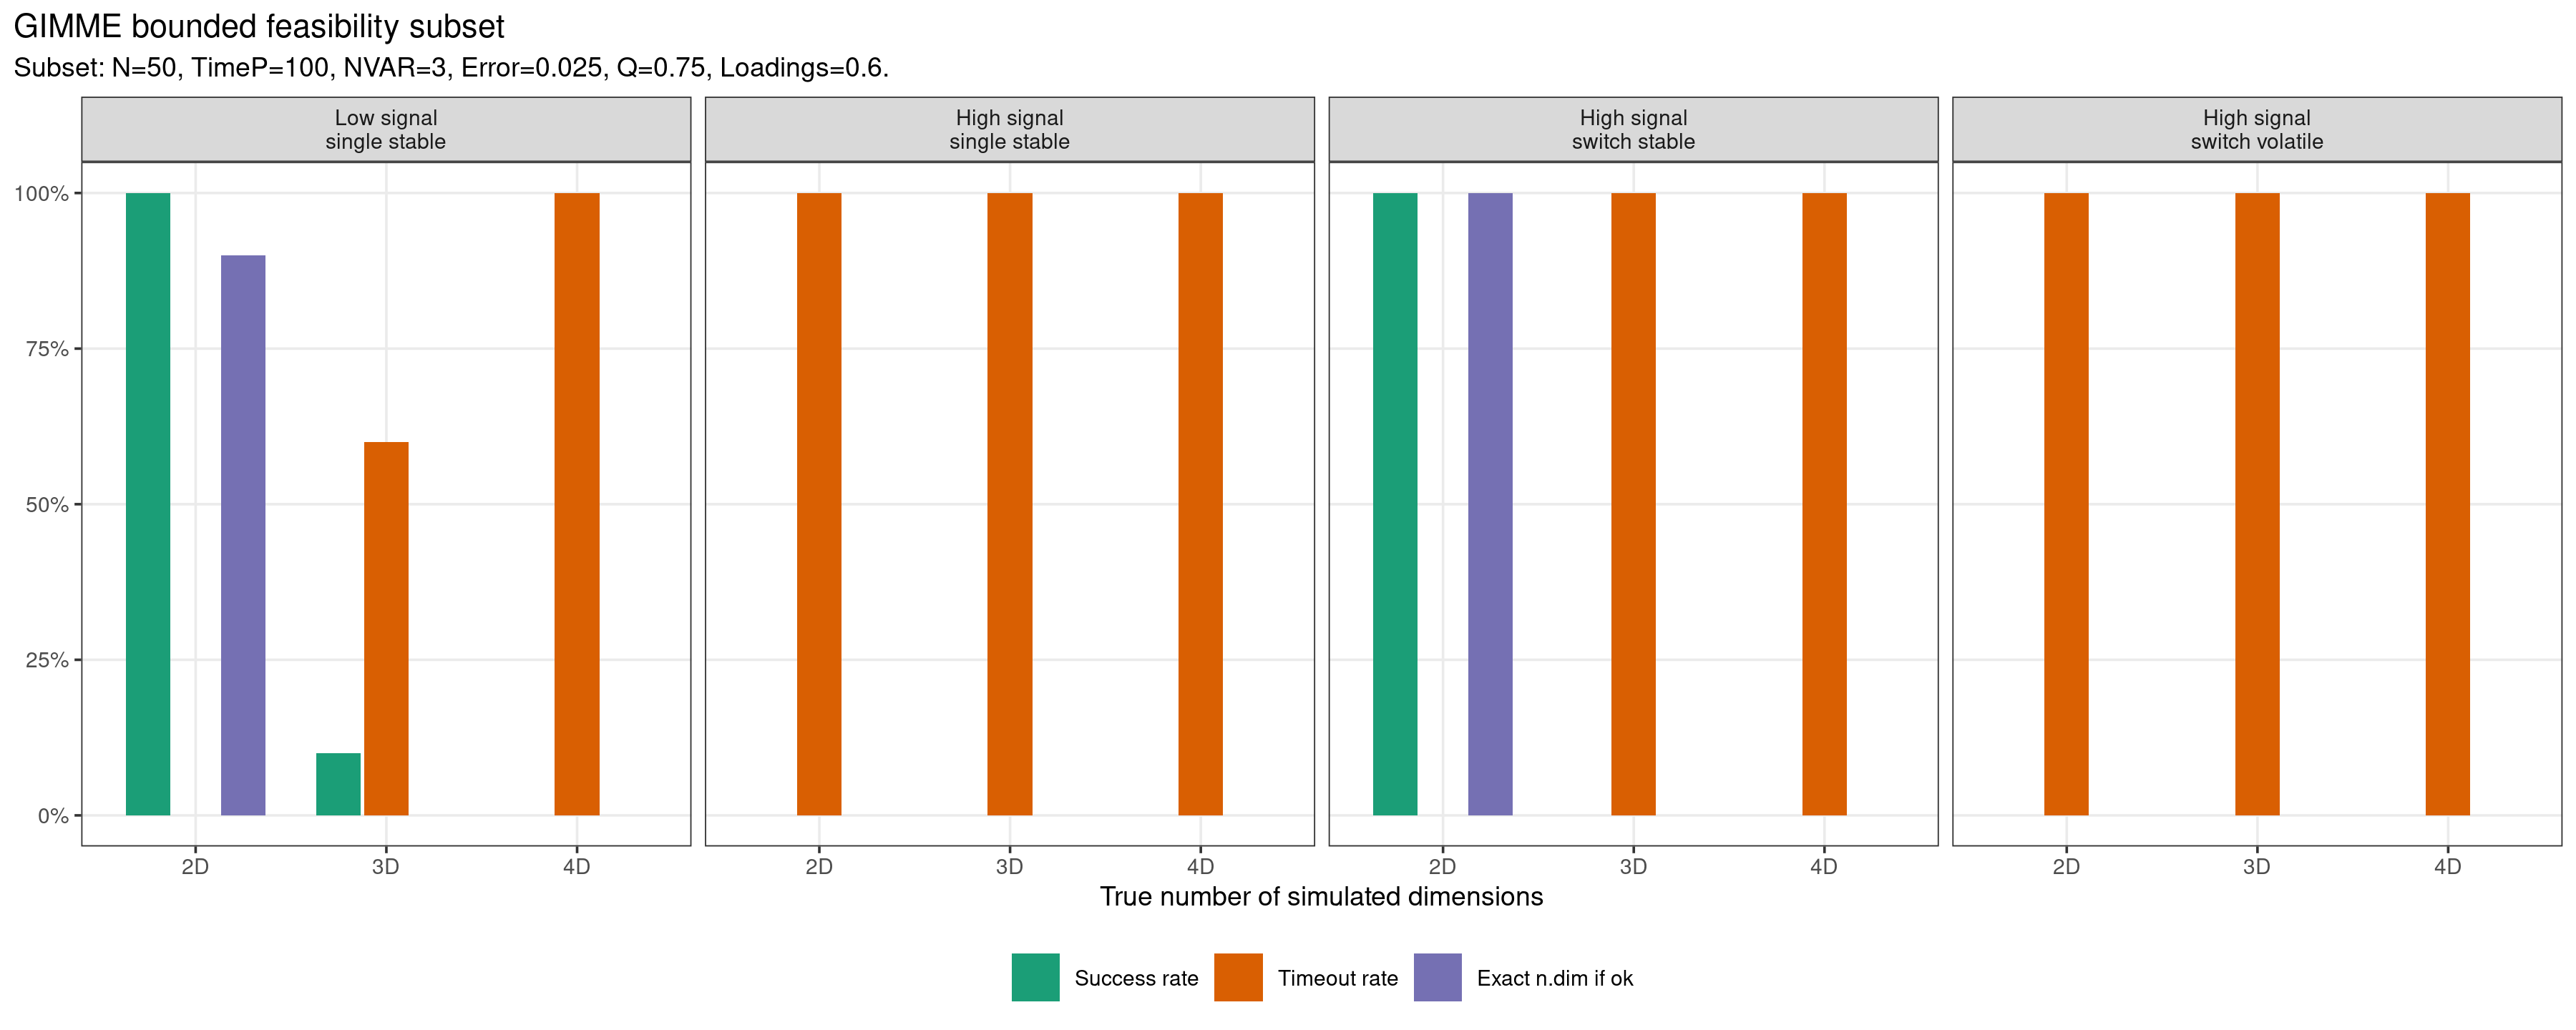
\includegraphics[width=0.92\linewidth]{comparison_revision_first_benchmark/05_gimme_bounded_feasibility.png}
\caption{Bounded GIMME feasibility results. GIMME is shown as a feasibility
analysis rather than a full-grid method because the same full design produced
unacceptable timeout rates.}
\label{fig:gimme-feasibility}
\end{figure}

\section{Empirical-Realism Check Against OAI-Large Time Series}

The second check asks whether the simulated panels have time-series properties
similar to observed OAI-large emotion-score series. The comparison uses the
MAFW OAI-large sample and the heterogeneous DLO synthetic panel. The current
similarity overview retained 86 observed base clips after empirical quality
control and compared them with synthetic panels collapsed to the same base-clip
level. The selected heterogeneous simulation used two latent factors with
$\eta=(-0.05,-0.15)$, $\zeta=(0.08,0.12)$, $\sigma_q=0.25$, and $dt=0.5$.

\begin{figure}[H]
\centering
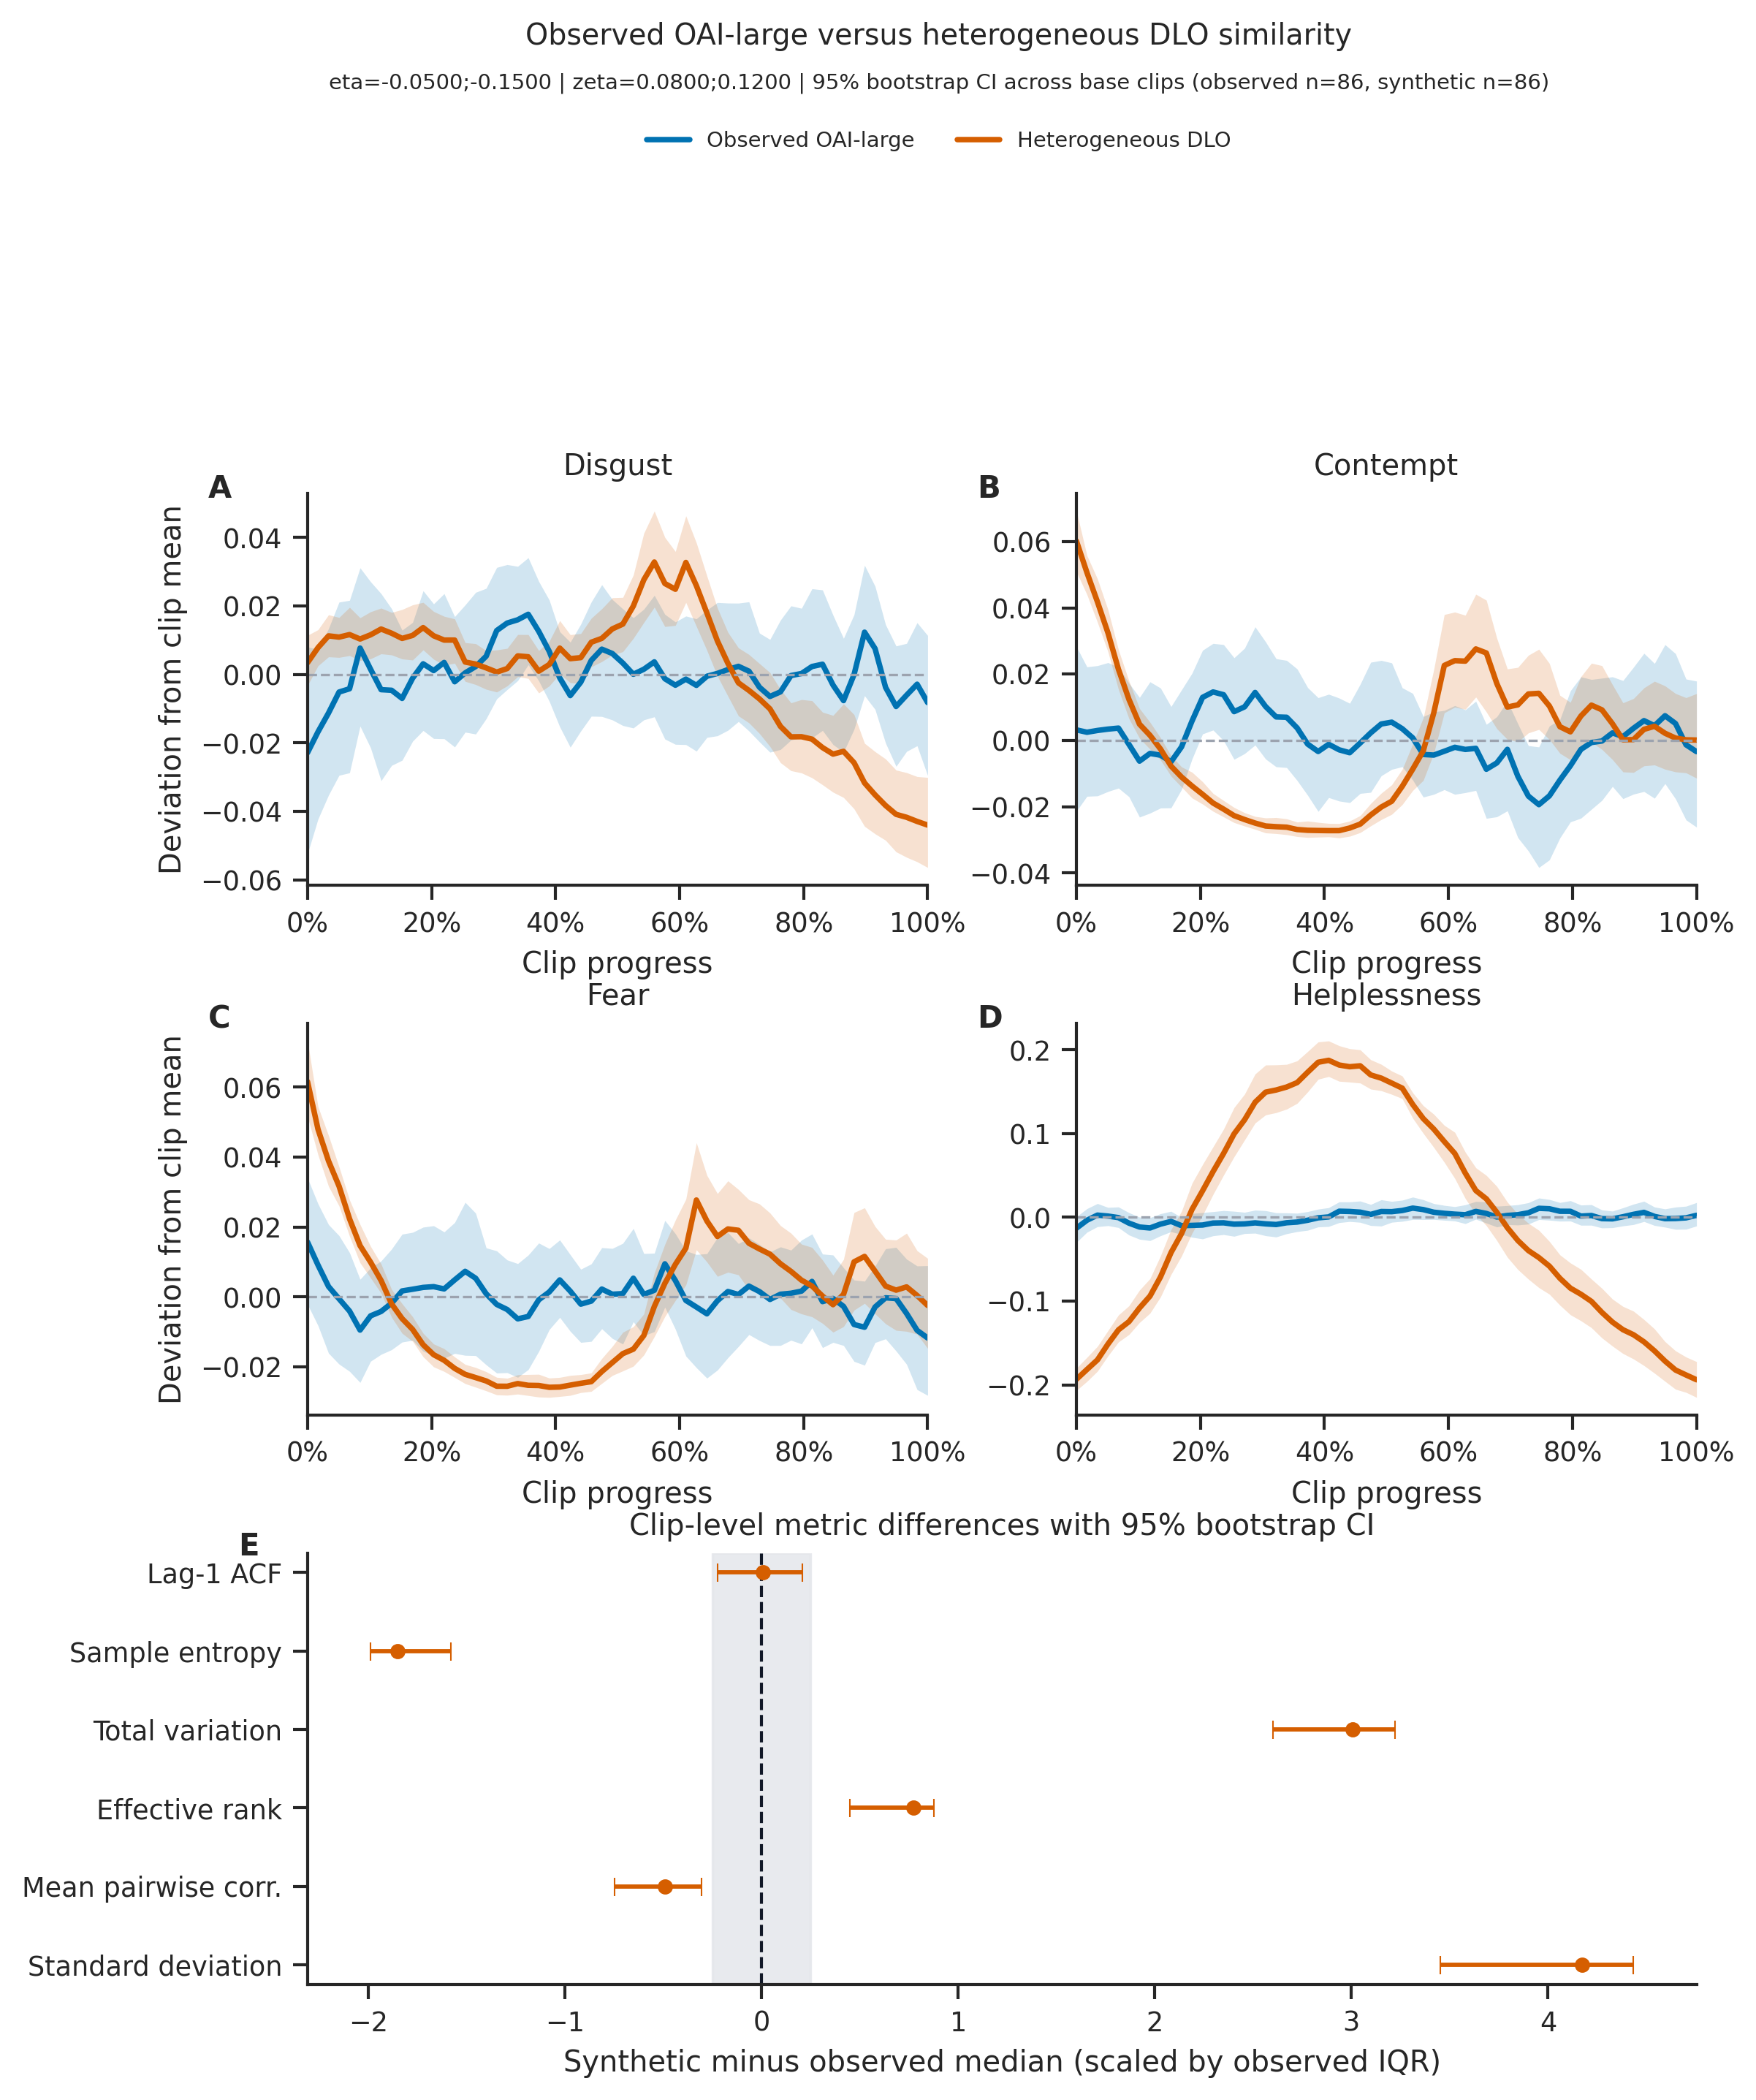
\includegraphics[width=0.92\linewidth]{empirical_outputs_smoke/mafw-sample/oai-large-100/heterogeneous_similarity_overview.png}
\caption{Observed OAI-large trajectories versus heterogeneous DLO simulations.
The bottom panel shows standardized median differences in raw time-series
metrics, scaled by the observed interquartile range.}
\label{fig:oai-similarity-overview}
\end{figure}

The entropy-oriented summary supports the basic empirical-realism claim: the
simulation is close to OAI-large on sample entropy, especially in the raw series
and reasonably in the latent score series. Other variability measures show
larger departures, especially standard deviation and total variation, so the
claim should be framed as partial realism rather than full distributional
equivalence.

\begin{table}[H]
\centering
\caption{Median variability properties for OAI-large empirical series and DLO
simulations. Values are medians from the 99-video OAI-large variability
calibration artifact.}
\label{tab:oai-entropy}
\small
\begin{tabular}{llrrr}
\toprule
Family & Metric & Empirical & DLO & Difference \\
\midrule
Raw & Sample entropy & 0.410 & 0.421 & 0.011 \\
Raw & Zero-crossing rate & 0.225 & 0.280 & 0.055 \\
Raw & Lag-1 ACF & 0.542 & 0.408 & -0.134 \\
Raw & Standard deviation & 0.020 & 0.090 & 0.070 \\
Raw & Total variation & 0.011 & 0.061 & 0.050 \\
\midrule
Latent & Sample entropy & 0.427 & 0.392 & -0.035 \\
Latent & Zero-crossing rate & 0.214 & 0.167 & -0.048 \\
Latent & Lag-1 ACF & 0.567 & 0.776 & 0.209 \\
Latent & Standard deviation & 0.321 & 1.570 & 1.249 \\
Latent & Total variation & 0.179 & 0.773 & 0.594 \\
\bottomrule
\end{tabular}
\end{table}

\section{Interpretation}

The revised comparison supports three conclusions. First, DynEGA is the best
default method for this design because it combines high dimensional recovery,
stable completion, and low runtime. Second, GraphicalVAR is a useful structural
comparator, but it is much more expensive and begins to fail in higher-dimensional
or more volatile scenarios. Third, GIMME should be presented as a bounded
feasibility sensitivity analysis rather than a primary benchmark competitor.

The empirical-realism checks indicate that the new DLO simulation can reproduce
some important OAI-large time-series properties, particularly entropy-like
irregularity measures. However, the synthetic panels still show larger movement
amplitudes and stronger latent smoothness than the empirical series. This is
acceptable for a method-recovery simulation, but it should be stated explicitly:
the generator is calibrated for plausible dynamic structure and entropy-like
behavior, not for exact reproduction of every marginal variability statistic.

\end{document}
